% Created 2023-11-16 Thu 13:08
% Intended LaTeX compiler: pdflatex
\documentclass[11pt]{article}
\usepackage[utf8]{inputenc}
\usepackage[T1]{fontenc}
\usepackage{graphicx}
\usepackage{longtable}
\usepackage{wrapfig}
\usepackage{rotating}
\usepackage[normalem]{ulem}
\usepackage{amsmath}
\usepackage{amssymb}
\usepackage{capt-of}
\usepackage{hyperref}
\usepackage{pgfplots}
\pgfplotsset{compat=1.18}
\author{Hankertrix}
\date{\today}
\title{Math Module 5B Cheat Sheet}
\hypersetup{
 pdfauthor={Hankertrix},
 pdftitle={Math Module 5B Cheat Sheet},
 pdfkeywords={},
 pdfsubject={},
 pdfcreator={Emacs 29.1 (Org mode 9.6.6)}, 
 pdflang={English}}
\begin{document}

\maketitle
\setcounter{tocdepth}{2}
\tableofcontents \clearpage
\section{Definitions}
\label{sec:org735af8b}

\subsection{Level sets}
\label{sec:org3abad53}
Consider a function \(f : D \rightarrow \mathbb{R}, D \subset \mathbb{R}^n\). For a given \(C \in \mathbb{R}\), the \textbf{level set} is the set of the form:
\[S = \{s \in D : f(x) = C\} \subset \mathbb{R}^n\]

\subsubsection{Example}
\label{sec:org8a8c62d}
\(F: \mathbb{R}^2 \rightarrow \mathbb{R}\) given by:

\begin{align*}
f(x, y) = x^2 + y^2, S &= \{(x, y) \in \mathbb{R}^2 : f(x, y) = 4\} \\
&= \{(x, y) \in \mathbb{R}^2 : x^2 + y^2 = 4\} \\
&= \text{a circle centred at } (0, 0) \text{ with radius } 2
\end{align*}

\newpage

\subsubsection{Common confusion}
\label{sec:org13c493a}
A level set of a function is \textbf{not} the same as the graph of a function. A level set can be thought of as a slice of the function at a particular value. The first figure below is the graph of the function \(x^2 + y^2\), and the second figure below is the level set \(x^2 + y^2 = 4\).

\begin{center}
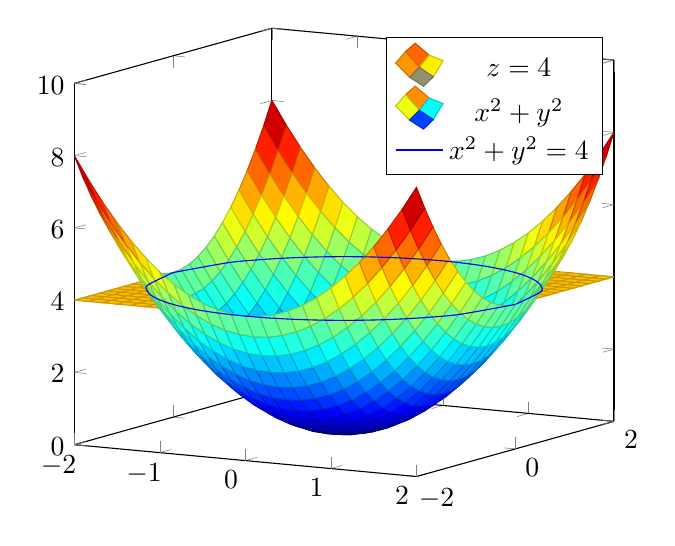
\begin{tikzpicture}
\begin{axis}[domain = -2:2, zmin = 0, zmax = 10, view = {30}{10}]

% The plane z = 4
\addplot3[surf]{4};
\addlegendentry{$z = 4$};

% The graph of x^2 + y^2
\addplot3[surf, colormap/jet]{x^2 + y^2};
\addlegendentry{$x^2 + y^2$};

% The graph of x^2 + y^2 = 4
\addplot3[draw = blue, smooth, samples y = 0]({x}, {sqrt(4 - x^2)}, 4);
\addplot3[draw = blue, smooth, samples y = 0]({x}, {-sqrt(4 - x^2)}, 4);
\addlegendentry{$x^2 + y^2 = 4$};

\end{axis}
\end{tikzpicture}

\[\]

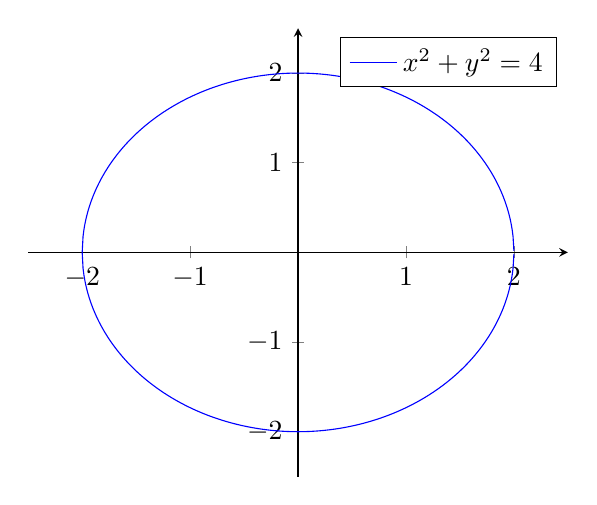
\begin{tikzpicture}
\begin{axis}[axis lines = center, domain = -2:2, samples = 500, xmin = -2.5, xmax = 2.5, ymin = -2.5, ymax = 2.5]

% The graph of x^2 + y^2 = 4
\addplot[color = blue]{sqrt(4 - x^2)};
\addplot[color = blue]{-sqrt(4 - x^2)};
\addlegendentry{$x^2 + y^2 = 4$};

\end{axis}
\end{tikzpicture}
\end{center}

\subsection{The restriction of a function}
\label{sec:orgced0e91}
Consider \(f : A \rightarrow \mathbb{R}\) and suppose \(B \subset A \subset \mathbb{R}^n\). The \textbf{restriction of \(f\) to \(B\)}, denoted by \(f|_B\), is the function with domain \(B\) given by:
\[f|_B = f(x), \quad \text{for } x \in B\]

\subsubsection{Example}
\label{sec:org043650f}
The function \(f(x) = \sin x\) is not increasing, but its restriction to \([\frac{\pi}{2}, \frac{\pi}{2}]\) is.

\begin{center}
\begin{tikzpicture}
\begin{axis}[axis lines = center, domain = -pi/2:pi/2, ymin = -1.2, ymax = 1.2]
\addplot[color = blue]{sin(deg(x))};
\end{axis}
\end{tikzpicture}
\end{center}

\subsubsection{Another example}
\label{sec:orgfb752a7}
Consider \(f : \mathbb{R}^2 \rightarrow \mathbb{R}\) given be \(f(x, y) = x^2 - y^2\). Take \(a, b \in \mathbb{R}\) and let:
\[A = \{(x, y) \in \mathbb{R}^2 : x = a\}, \quad B = \{(x, y) \in \mathbb{R}^2 : y = b\}\]

Then:
\[f|_A (x, y) = f(a, y) = a^2 - y^2, \quad f|_B (x, y) = f(x, b) = x^2 - b^2\]

Note that the restricted functions \(f|_A\) and \(f|_B\) become one-variable functions.
\\[0pt]

\textbf{Simplified notation}:
\[f|_{x = a} \text{ instead of } f|_{\{(x, y) \in \mathbb{R}^2 : x = a\}}\]

\subsection{Limit points}
\label{sec:org2939b07}
Let \(A\) be a subset of \(\mathbb{R}^n\). We say that a point \(\boldsymbol{a} \in mathbb{R}^n\) is a \textbf{limit point} of \(A\), if for every \(\delta > 0\), there exists a point \(\boldsymbol{x} \in A\) such that \(0 < ||x - \boldsymbol{a}|| < \delta\).

\subsection{Limits}
\label{sec:org3c24e86}
Consider \(f : A \rightarrow \mathbb{R}^m, A \subset \mathbb{R}^n\) and suppose \(\boldsymbol{a}\) is a limit point of \(A\). We say that \(f\) approaches a \textbf{limit} \(\boldsymbol{L}\) as \(\boldsymbol{x}\) approaches \(\boldsymbol{a}\) and write \(\lim_{x \rightarrow a} f(\boldsymbol{x}) = \boldsymbol{L}\) if for every \(\varepsilon > 0\), there exists a \(\delta > 0\) such that:
\[0 < ||\boldsymbol{x} - \boldsymbol{a}|| < \delta, \quad \boldsymbol{x} \in A \Rightarrow ||f(\boldsymbol{x}) - \boldsymbol{L}|| < \varepsilon\]

\[\lim_{\boldsymbol{x} \rightarrow \boldsymbol{a}} f(\boldsymbol{x}) = \boldsymbol{L} \quad \Leftrightarrow \quad \lim_{\boldsymbol{x} \rightarrow \boldsymbol{a}} ||f(\boldsymbol{x}) - \boldsymbol{L}|| = 0\]

\subsection{Squeeze theorem}
\label{sec:orgc52a3c9}
For \textbf{real valued} functions (functions whose codomain is \(\mathbb{R}\)), we have a result analogous to the one variable squeeze theorem.
\\[0pt]

Consider \(f, g, h : A \rightarrow \mathbb{R}, A \subset \mathbb{R}^n\). Suppose there exists \(\delta > 0\) such that:
\[f(\boldsymbol{x}) \le g(\boldsymbol{x}) \le h(\boldsymbol{x}), \quad \text{for } 0 < ||\boldsymbol{x} - \boldsymbol{a}|| < \delta, \quad \boldsymbol{x} \in A\]

Then:
\[\lim_{\boldsymbol{x} \rightarrow \boldsymbol{a}} f(\boldsymbol{x}) = \lim_{\boldsymbol{x} \rightarrow \boldsymbol{a}} h(\boldsymbol{x}) = L \quad \Rightarrow \quad \lim_{\boldsymbol{x} \rightarrow \boldsymbol{a}} g(\boldsymbol{x}) = L\]

\subsection{A useful inequality}
\label{sec:org224eac9}
Take \(\boldsymbol{x} = (x_1, x_2, \ldots, x_n) \in \mathbb{R}^n\). Then:
\[|x_i| \le ||\boldsymbol{x}||, \text{ for } i = 1, 2, \ldots, n\]

\subsubsection{Proof}
\label{sec:org5e27886}
\[|x_i| = \sqrt{x_i^2} \le \sqrt{x_1^2 + x_2^2 + \ldots + x_n^2} = ||\boldsymbol{x}||\]

\subsection{Components of vector valued functions}
\label{sec:org9e2fa43}
Suppose \(f : A \rightarrow \mathbb{R}^m, A \in \mathbb{R}^n, m \ge 2\). In other words, for \(\boldsymbol{x} \in A\), we have \(f(\boldsymbol{x}) \in \mathbb{R}^m\). This means that we can express \(f(\boldsymbol{x})\) as:
\[f(\boldsymbol{x}) = (f_1(\boldsymbol{x}), f_2(\boldsymbol{x})), \ldots, f_m(\boldsymbol{x})\]

Where:
\[f_1, f_2, \ldots, f_m : A \rightarrow \mathbb{R}\]

The functions \(f_i i = 1, \ldots, m\) are called the \textbf{component functions} of \(f\).

\subsubsection{Example}
\label{sec:org5743431}
The function \(f : \mathbb{R}^3 \rightarrow \mathbb{R}^2\), given by:
\[f(x, y, z) = (x + z, 2y^2)\]

Has component functions:
\[f_1(x, y, z) = x + z, \quad f_2(x, y, z) = 2y^2\]

Note that while \(f\) is vector valued, the component functions are both scalar valued (real valued).

\subsection{Limits of vector valued functions}
\label{sec:org0933023}
For vector valued functions, we can evaluate limits component-wise. Consider \(f : A \rightarrow \mathbb{R}^m, A \subset \mathbb{R}^n\) and let \(\boldsymbol{a}\) be a limit point of \(A\). Let \(\boldsymbol{L} = (L_1, L_2, \ldots, L_m) \in \mathbb{R}^m\) and let \(f_1, f_2, \ldots, f_m\) be the component functions of \(f\). Then:

\[\lim_{\boldsymbol{x} \rightarrow \boldsymbol{a}} f(x) = \boldsymbol{L}\]

If and only if:
\[\lim_{\boldsymbol{x} \rightarrow \boldsymbol{a}} f_i (\boldsymbol{x}) = L_i, \quad \text{for all } i = 1, \ldots, m\]

Basically, the theorem simply states:
\[\lim_{\boldsymbol{x} \rightarrow \boldsymbol{a}} (f_1 (\boldsymbol{x}), f_2(\boldsymbol{x}), \ldots, f_m(\boldsymbol{x})) = \left(\lim_{\boldsymbol{x} \rightarrow \boldsymbol{a}} f_1(\boldsymbol{x}), \lim_{\boldsymbol{x} \rightarrow \boldsymbol{a}} f_2 (\boldsymbol{x}), \ldots, \lim_{\boldsymbol{x} \rightarrow \boldsymbol{a}} f_m (\boldsymbol{x}) \right)\]

\subsection{Continuity}
\label{sec:orgac7abab}
We say that a function \(f : A \rightarrow \mathbb{R}^m, A \subset \mathbb{R}^n\), is *continuous at \(\boldsymbol{a} \in A\) if any \(\varepsilon > 0\), there exists a \(\delta > 0\) such that:
\[||\boldsymbol{x} - \boldsymbol{a}|| < \delta, \ \boldsymbol{x} \in A \quad \Rightarrow \quad ||f(\boldsymbol{x}) - f(\boldsymbol{a})|| < \varepsilon\]

If \(B \subset A\) and \(f\) is continuous at every \(\boldsymbol{a} \in B\), we say that \(f\) is \textbf{continuous on \(B\)}. If \(f\) is continuous on \(A\), we say that \(f\) is \textbf{continuous}.

\subsubsection{Theorem}
\label{sec:org503f883}
Consider a function \(f : A \rightarrow \mathbb{R}^m\) and suppose \(\boldsymbol{a} \in A\) is also a limit point of \(A\). Then \(f\) is continuous at \(\boldsymbol{a}\) if and only if:
\[\lim_{\boldsymbol{x} \rightarrow \boldsymbol{a}} = f(\boldsymbol{a})\]

\subsection{One-sided limits}
\label{sec:orge689877}
If \(f\) is defined both to the left and right of \(a\), we have
\[\lim_{x \rightarrow a} f(x) = L \quad \Rightarrow \quad \lim_{x \rightarrow a-} f(x) = \lim_{x \rightarrow a+} f(x) = L\]

\subsection{Limit of sequences}
\label{sec:org043cfc4}
Suppose a is a limit point of \(f\)'s domain and consider a sequence \(a_n \rightarrow a\) as \(n \rightarrow \infty\). Then:
\[\lim_{x \rightarrow a} f(x) = L \quad \Rightarrow \quad \lim_{n \rightarrow \infty} f(a_n) = L\]

\newpage

\subsection{Limits of restrictions}
\label{sec:org2a864a9}
Consider \(f : A \rightarrow \mathbb{R}^m, A \subset \mathbb{R}^n\), a subset \(B \subset A\), and a limit point \(\boldsymbol{a}\) of \(B\) (consequently \(\boldsymbol{a}\) is also a limit point of \(A\)). Then:
\[\lim_{\boldsymbol{x} \rightarrow \boldsymbol{a}} f(\boldsymbol{x}) = \boldsymbol{L} \quad \Rightarrow \quad \lim_{\boldsymbol{x} \rightarrow \boldsymbol{a}} f|_B(\boldsymbol{x}) = \boldsymbol{L}\]

\subsubsection{How to use the theorem}
\label{sec:org8ec494a}
Consider \(f : A \rightarrow \mathbb{R}^m, A \subset \mathbb{R}^n\), and two subsets \(B_1 \subset A, B_2 \subset A\). The previous theorem tells us that:
\[\lim_{\boldsymbol{x} \rightarrow \boldsymbol{a}} f(\boldsymbol{x}) = \boldsymbol{L} \quad \rightarrow \quad \lim_{\boldsymbol{x} \rightarrow \boldsymbol{a}} f|_{B_1} (\boldsymbol{x}) = \lim_{\boldsymbol{x} \rightarrow \boldsymbol{a}} f|_{B_2}(\boldsymbol{x}) = \boldsymbol{L}\]

Loosely speaking, if the left limit exists, we must have the same limit whichever way we approach \(\boldsymbol{a}\).
\\[0pt]

Hence, if we can find subsets \(B_1, B_2 \subset A\) such that:
\[\lim_{\boldsymbol{x} \rightarrow \boldsymbol{a}} f|_{B_1}(\boldsymbol{x}) \ne \lim_{\boldsymbol{x} \rightarrow \boldsymbol{a}} f|_{B_2} (\boldsymbol{x})\]

We can conclude that:
\[\lim_{\boldsymbol{x} \rightarrow \boldsymbol{a}} f(\boldsymbol{x}) \text{ does not exist}\]

\newpage

\subsection{Partial derivatives}
\label{sec:org18da805}
Consider \(f : A \rightarrow \mathbb{R}, A \subset \mathbb{R}^n\). The partial derivative \(f_{x_k} (a_1, a_2, \ldots, a_n)\) with respect to \(x_k\) of \(f(x_1, x_2, \ldots, x_n)\) at the point \(\boldsymbol{a} = (a_1, a_2, \ldots, a_n) \in A\), given the derivative exists, is:
\[f_{x_k}(a_1, a_2, \ldots, a_n) = \frac{d}{dt} f(a_1, \ldots, a_{k - 1}, t, a_{k + 1}, \ldots, a_n)|_{t = a_k}\]

Another common notation for the partial derivative \(f_{x_k}\) is:
\[\frac{\partial f}{\partial x_k}\]

\subsubsection{Calculating partial derivatives}
\label{sec:org941dbec}
Since a partial derivative is just our usual one variable derivative (we consider all but one variable constant and differentiate the one variable function we get), all the differentiation rules still hold.
\\[0pt]

In other words: \textbf{Just think of the other variables as constants and differentiate as usual}.

\subsubsection{Example 1}
\label{sec:org581ed2e}
With \(f(x, y) = x^2 + y^2\) we get:
\[f_x(x, y) = 2x, \quad f_y(x, y) = -2y\]

In particular:
\[f_x(1, -2) = 2 \cdot 1 = 2, f_y (1, -2) = -2 \cdot (-2) = 4\]

\subsubsection{Example 2}
\label{sec:orgffa6936}
For \(f(x, y, z) = \sin (xyz) + x^2 y\), we have:
\begin{align}
f_x(x, y, z) &= yz \cos (xyz) + 2xy, \\
f_y(x, y, z) &= xz \cos (xyz) + x^2, \\
f_z(x, y, z) &= xy \cos (xyz)
\end{align}

\subsubsection{One variable example}
\label{sec:org01044cd}
However, even in one variable, the differentiation rules don't always apply. For example, what is wrong with the following argument?
\\[0pt]

Let:
\[
f(x) = |x| = \begin{cases}
x & \text{for } x \ge 0 \\
-x & \text{for } x < 0
\end{cases}
\]

Hence:
\begin{align*}
f'(0) &= \frac{df}{dx}|_{x = 0} \\
&= \frac{d}{dx}x|_{x = 0} \\
&= 1|_{x = 0} \\
&= 1
\end{align*}

However, this is wrong, as:
\begin{align*}
f'(0) &= \lim_{h \rightarrow 0} \frac{f(0 + h) - f(0)}{h} \\
&= \lim_{h \rightarrow 0} \frac{|h|}{h} \text{ does not exist}
\end{align*}

Because:
\begin{align*}
\lim_{h \rightarrow 0+} \frac{|h|}{h} &= \lim_{h \rightarrow 0} \frac{h}{h} \\
&= 1
\end{align*}

\begin{align*}
\lim_{h \rightarrow 0-} \frac{|h|}{h} &= \lim_{h \rightarrow 0} \frac{-h}{h} \\
&= -1
\end{align*}

Since \(\lim_{h \rightarrow 0-} \frac{|h|}{h} \ne \lim_{h \rightarrow 0+} \frac{|h|}{h}\), the limit does not exist.

\newpage

\subsubsection{Two variable example}
\label{sec:orgbf4da7c}
Let:
\[
f(x, y) = \begin{cases}
\frac{x^3}{x^2 + y^2} & \text{for } (x, y) \ne (0, 0) \\
0 & \text{for } (x, y) = (0, 0)
\end{cases}
\]


Evaluate:

\[
f(x, 0) = \begin{cases}
\frac{x^3}{x^2 + 0^2} = x & \text{for } x \ne 0 \\
0 & \text{for } x = 0
\end{cases}
\quad = x \text{ for all } x \tag{1}
\]

\begin{align*}
f_x(0, 0) &= \frac{d}{dx} f(x, 0)|_{x = 0} \\
&= \frac{d}{dx}x|_{x = 0} \quad \because (1) \\
&= 1|_{x = 0} \\
&= 1
\end{align*}

\[
f(0, y) = \begin{cases}
\frac{0}{0^2 + y^2} = 0 & \text{for } y \ne 0 \\
0 & \text{for } y = 0
\end{cases}
\quad = 0 \text{ for all } y \tag{2}
\]

\begin{align*}
f_y(0, 0) &= \frac{d}{dy} f(0, y)|_{x = 0} \\
&= \frac{d}{dy}0|_{x = 0} \quad \because (2) \\
&= 0|_{x = 1} \\
&= 0
\end{align*}

\subsection{Clairaut's theorem}
\label{sec:org06ac5bc}
Consider \(f : A \rightarrow \mathbb{R}, A \subset \mathbb{R}^n\). Suppose that for some \(\delta > 0\), the functions \(f_{x_j x_k} (\boldsymbol{x})\) and \(f_{x_k x_j} (\boldsymbol{x})\) are both continuous on:
\[\{x \in \mathbb{R}^n : ||\boldsymbol{x} - \boldsymbol{a}|| < \delta\}\]

Then:
\[f_{x_j x_k} (\boldsymbol{a}) = f_{x_k x_j}(\boldsymbol{a})\]

\subsubsection{Higher order derivatives}
\label{sec:org53faba1}
The theorem can be generalised to higher order derivatives. If two mixed partial derivatives with the same number of differentiations with respect to the same variables, are continuous \(\boldsymbol{a}\), then they are equal at \(\boldsymbol{a}\). For example:

\[f_{zzyzxyx} (a, b, c) = f_{xxyyzzz} (a, b, c)\]
If both are continuous near \((a, b, c)\).


\section{Limit laws}
\label{sec:orgd705e5a}
For \(f, g : A \rightarrow \mathbb{R}^m, A \subset \mathbb{R}^n\), a limit point \(\boldsymbol{a}\) of \(A\), \(C_1, C_2, p \in \mathbb{R}\) and if the \textbf{right-hand side exists}, we have:

\[\text{1. } \lim_{\boldsymbol{x} \rightarrow \boldsymbol{a}} [C_1 f(\boldsymbol{x}) + C_2 g(\boldsymbol{x})] = C_1 \lim_{\boldsymbol{x} \rightarrow \boldsymbol{a}} f(\boldsymbol{x}) + C_2 \lim_{\boldsymbol{x} \rightarrow \boldsymbol{a}} g(\boldsymbol{x})\]
\[\text{2. } \lim_{\boldsymbol{x} \rightarrow \boldsymbol{a}} [f(\boldsymbol{x}) g(\boldsymbol{x})] = \lim_{\boldsymbol{x} \rightarrow \boldsymbol{a}} f(\boldsymbol{x}) \cdot \lim_{\boldsymbol{x} \rightarrow \boldsymbol{a}} g(\boldsymbol{x})\]
\[\text{3. } \lim_{\boldsymbol{x} \rightarrow \boldsymbol{a}} [f(\boldsymbol{x})]^p = \left[\lim_{\boldsymbol{x} \rightarrow \boldsymbol{a}} f(\boldsymbol{x}) \right]^p\]

\subsection{Composition rule}
\label{sec:org92177a1}
Suppose \(\lim_{\boldsymbol{x} \rightarrow \boldsymbol{a}} g(\boldsymbol{x}) = \boldsymbol{L}\) and suppose that \(f(\boldsymbol{x})\) is continuous at \(\boldsymbol{x} = \boldsymbol{L}\). Then:
\[\lim_{\boldsymbol{x} \rightarrow \boldsymbol{a}} f(g(\boldsymbol{x})) = f(L)\]

In other words, for continuous \(f\) we have:
\[\lim_{\boldsymbol{x} \rightarrow \boldsymbol{a}} f(g(\boldsymbol{x})) = f \left(\lim_{\boldsymbol{x} \rightarrow \boldsymbol{a}} g(\boldsymbol{x}) \right)\]

\newpage

\section{Second order partial derivatives}
\label{sec:org34019e3}
Since \(f_x(x, y)\) and \(f_y(x, y)\) are also functions of \(x\) and \(y\), we can consider partial derivatives of those functions.
\\[0pt]

Notation:
\\[0pt]

\(\frac{\partial}{\partial x} f_x (x, y)\) is also denoted \(\frac{\partial^2 f}{\partial x^2}\) or \(f_{xx}(x, y)\).
\\[0pt]

\(\frac{\partial}{\partial y} f_x (x, y)\) is also denoted \(\frac{\partial^2 f}{\partial y \partial x}\) or \(f_{xy}(x, y)\).
\\[0pt]

\(\frac{\partial}{\partial x} f_y (x, y)\) is also denoted \(\frac{\partial^2 f}{\partial x \partial y}\) or \(f_{yx}(x, y)\).
\\[0pt]

\(\frac{\partial}{\partial y} f_y (x, y)\) is also denoted \(\frac{\partial^2 f}{\partial y^2}\) or \(f_{yy}(x, y)\).
\\[0pt]

\(f_{xy}\) and \(f_{yx}\) are called \textbf{mixed} partial derivatives.
\end{document}